\section {Evaluation\\}
 
In this section, we conducted experiments to evaluate the performance of 
several web-based event\footnote{the term ``event" here refers to the ``latest 
updates in the server side", which differs from the meaning in ``event-driven"
} notification mechanisms. We also evaluated PushUp servers' performance with
different server numbers.

To better characterize the performance of the PushUp server, we chose ``Client
Pulling" and ``Multithreadeding long polling" as the baseline. The PushUp
adopted the Event-driven long polling mechanism.

\begin{itemize}
    \item {\bf Client Pulling (CP): } In this method the client side initiates 
        an http request to the server to pull the latest updates on a regular 
        basis.
    \item {\bf Multithreadeding long polling(MLP): } This method realizes the 
        long polling by multi threads. For each incoming polling request, the
        server will create a thread waiting for the latest updates.
    \item {\bf Event-driven long polling(ELP): } This method realizes the long
        polling by event-driven mechanism. This method keeps all the polling 
        requests within a single thread.
\end{itemize}

\subsection{Settings \\}

\subsubsection{Evaluation Metrics \\}
In the evaluation, we used the following control variables to control in
the experiments.

\begin{itemize}
    \item {\bf Number of concurrent connections}: This variable allows us 
         to evaluate the scalability of different methods.
    \item {\bf Publish Interval}: This variable controls the frequency of 
         event publication by the server. 
    \item {\bf Polling interval}: This variable determines how long will 
        the method send a polling request to the server. For client 
        pulling, it sends polling request at a regular basis; as for
        long polling methods, they send polling request (1) after they
        just received a new update or (2) after a suitable timeout.
\end{itemize}

And we used the following metrics to evaluate the performance of different
methods.
\begin{itemize}
    \item {\bf Network Traffic (NT)}: NT evaluates the network usage for
        different event notification methods.
    \item {\bf Mean Publish Trip Time (MPT)}: The publish trip-time is 
        the time elapsed between the creation of a data by the server and 
        its reception by the client. It shows how long it takes for the 
        client to be updated when an event occurs.
    \item {\bf Received Message Percentage (RMP)}: RMP indicates the data 
        loss in during the network communication. 
    \item {\bf Server Memory Usage (SMU)}: In many real world long polling 
        system, the polling requests spent most of their time waiting for 
        the new events.[source needed] Thus, memory cost for each idle 
        polling requests is critical to the overall performance.
\end{itemize}

\subsubsection{Evaluation Environment \\}
The experiments are done in CMU's PEACE cluster. Each machine in the cluster 
has a 4 CPU cores(AMD Opteron Processor 4130, 2600 MHz, 512K cache size),
8 GB RAM and 1 physical 581 GB disk.

\subsection{Push Model vs. Poll Model\\}

One of the biggest advantage of long polling strategy is its significant 
reduction of network traffic (due to the reduced overhead in creating connections).
In the following experiments we focused on the evaluation on the network 
traffic(NT) and mean publish trip time(MPT).

Since the goal of these experiments is to characterize the network traffic 
of different methods. We evaluated the {\bf network traffic} and {\bf mean 
publish trip time} only with some moderate number of concurrent 
connections: 10, 100 and 1000. 

The {\bf publish time} are $10 sec$, $20 sec$, $30 sec$, $40 sec$ and 
$50 sec$. The {\bf polling time} we chose for the {\bf client pulling}
is $1 sec$, and $50 sec$ for long polling based methods(which is a 
popular choice in real world long polling applications).

Table \ref{tb:traffic} shows the detailed network traffic with different 
publish time and number of concurrent connections (written as ``cc" 
in the tables).  We can see that the long polling based method keeps 
a relatively constant network traffic while the client pull method's 
network traffic grows (almost) linearly as the publish time increases.
Figure \ref{fig:traffic} shows the network traffic change when the number 
of concurrent connection is $1000$.

Table \ref{tb:mpt_all} demonstrates the mean publish trip time with 
different publish time and number of concurrent connections. The MPT of
client pull increases much faster than the long polling based methods.
This could be caused by the increase in growing network traffic which lead to a 
higher chance of package loss in the client pull method. 
Figure \ref{fig:traffic_latency} compares the MPT of push and pull models when 
the number of concurrent connection is $1000$.

In summary, the push model significantly reduce the network traffic, which in
turn, yields a smaller mean publish trip time as the concurrent connections 
increase. 

Also, we observed that the multithreading-based long polling and event-driven long 
polling have similar performance in terms of network traffic and mean publish
trip time when the number of concurrent connections is relatively small. In the 
next evaluation we will test both long polling methods' performance with large 
concurrent connections.

\begin{table}
\centering \caption{\label{tb:traffic} Network Traffic(KB)}
\begin{tabular}{|l|l|l|l|l|l|}
    \hline cc=10& 10 sec & 20 sec & 30 sec & 40 sec & 50 sec \\
    \hline CP & 12.7 & 25.8 & 39.8 & 55.2 & 68.2 \\
    \hline MLP & 1.27 & 1.27 & 1.27 & 1.27 & 1.27 \\
    \hline ELP & 1.27 & 1.27 & 1.27 & 1.27 & 1.27 \\
    \hline
    \hline cc=100& 10 sec & 20 sec & 30 sec & 40 sec & 50 sec \\
    \hline CP & 127.4 & 277.1 & 415.2 & 580.5 & 745.5 \\
    \hline MLP & 12.7 & 12.7 & 12.7 & 12.7 & 13.1 \\
    \hline ELP & 12.7 & 12.7 & 12.7 & 12.7 & 12.7 \\
    \hline
    \hline cc=1000 & 10 sec & 20 sec & 30 sec & 40 sec & 50 sec \\
    \hline CP & 1370.5 & 3457.1 & 5537.5 & 7282.5 & 10743.5 \\
    \hline MLP & 135.5 & 132.5 & 137.8 & 133.4 & 135.5 \\
    \hline ELP & 130.1 & 129.5 & 132.8 & 131.8 & 130.5 \\
    \hline
\end{tabular}
\end{table}

\begin{figure}[htb!]
\centering%
    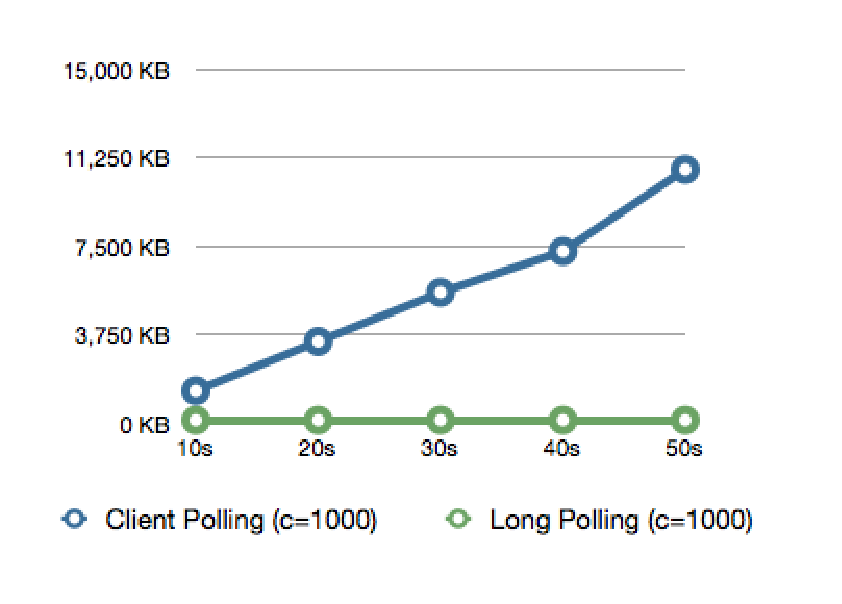
\includegraphics[scale=0.70]{figures/io.eps}
    \caption{Network Traffic of Pull \& Push Models}
    \label{fig:traffic}
\end{figure}


\begin{table}
\centering \caption{\label{tb:mpt_all} Mean Publish Trip Time (second)}
\begin{tabular}{|l|l|l|l|l|l|}
    \hline cc=10 & 10 sec & 20 sec & 30 sec & 40 sec & 50 sec \\
    \hline CP & 0.6 & 0.7 & 0.5 & 0.7 & 0.8 \\
    \hline MLP & 0.1 & 0.0 & 0.1 & 0.2 & 0.1 \\
    \hline ELP & 0.2 & 0.1 & 0.1 & 0.4 & 0.2 \\
    \hline
    \hline cc=100 & 10 sec & 20 sec & 30 sec & 40 sec & 50 sec \\
    \hline CP & 0.8 & 1.1 & 2.5 & 3.1 & 2.7 \\
    \hline MLP & 0.5 & 0.4 & 0.5 & 0.8 & 1.1 \\
    \hline ELP & 0.7 & 0.4 & 0.8 & 1.2 & 0.9 \\
    \hline
    \hline cc=1000& 10 sec & 20 sec & 30 sec & 40 sec & 50 sec \\
    \hline CP & 2.8 & 3.4 & 4.5 & 5.3 & 7.2 \\
    \hline MLP & 2.3 & 2.9 & 2.7 & 3.5 & 3.4 \\
    \hline ELP & 2.4 & 2.8 & 1.8 & 2.4 & 2.9 \\
    \hline
\end{tabular}
\end{table}

\begin{figure}[htb!]
\centering%
    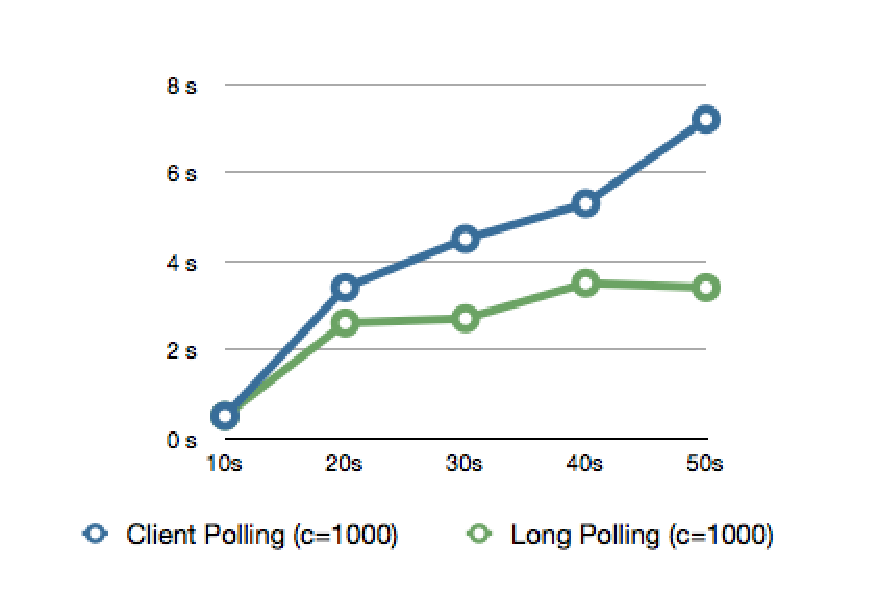
\includegraphics[scale=0.70]{figures/latency.eps}
    \caption{Mean Publish Trip Time of Pull \& Push Models}
    \label{fig:traffic_latency}
\end{figure}

\subsection{Event vs. Thread\\}

Here we compared the performance between event-driven long polling method
and the multithreading long polling method. In the following evaluation
we tested the {\bf server memory usage(SMU)}, {\bf mean publish trip time
(MPT)}, {\bf received message percentage(RMP)} with a larger number of
active connections(from 500-16000).

Figure \ref{fig:et_memory} shows the server memory usage of both methods.
The event-driven method demonstrates an excellent memory usage as the
number of active connections increases, while the memory usage of 
multithreading method soars rapidly and reaches $100\%$ when the active
connections' number goes to $8000$.

Figure \ref{fig:et_latency} and figure \ref{fig:et_rate}, show the mean
publish trip time and received message percentage. Event-driven method 
significantly excels multithreading method in both evaluation.

Thus we believe that one-polling-request-per-thread approach is not a good 
choice for handling large amount of concurrent connections, as its
memory usage and possible context switch may incur very large overhead.
The event-driven method, on the other hand, demonstrates a better 
memory usage and while supporting the same number of clients.  

\begin{figure}[htb!]
\centering%
    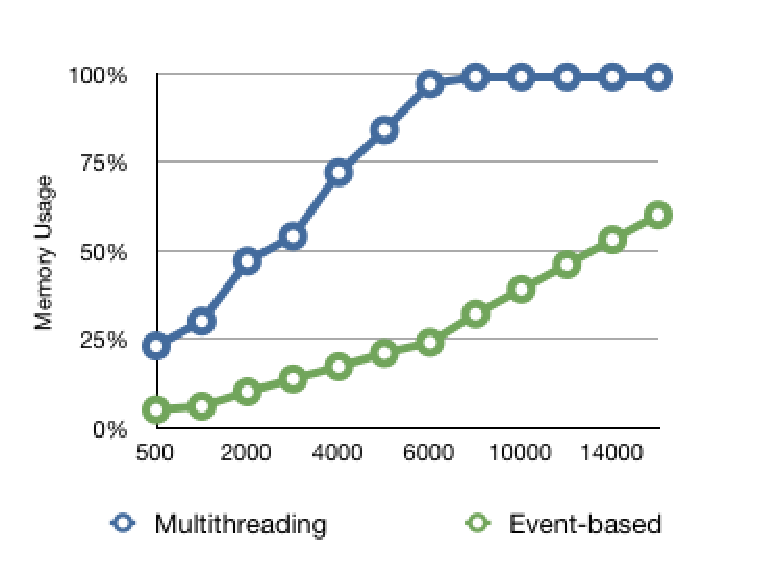
\includegraphics[scale=0.70]{figures/et_memory.eps}
    \caption{Server Memory Usage}
    \label{fig:et_memory}
\end{figure}

\begin{figure}[htb!]
\centering%
    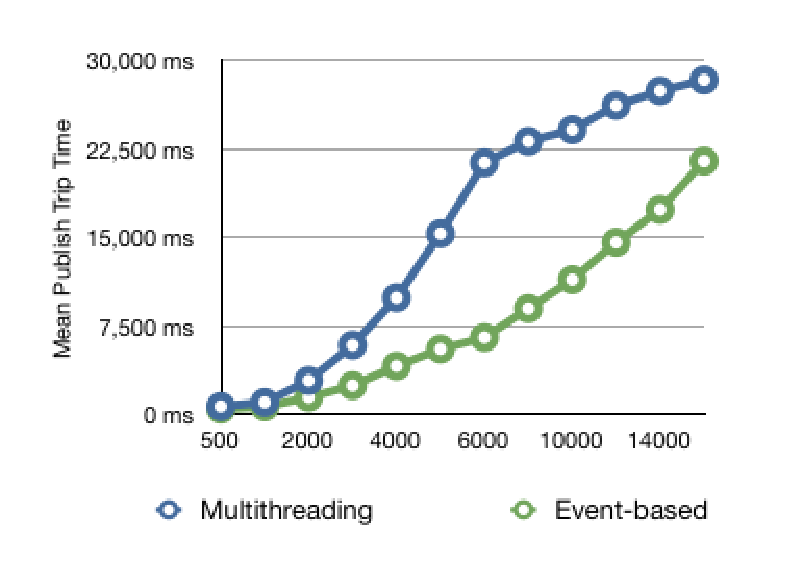
\includegraphics[scale=0.70]{figures/et_latency.eps}
    \caption{Mean Publish Trip Time}
    \label{fig:et_latency}
\end{figure}

\begin{figure}[htb!]
\centering%
    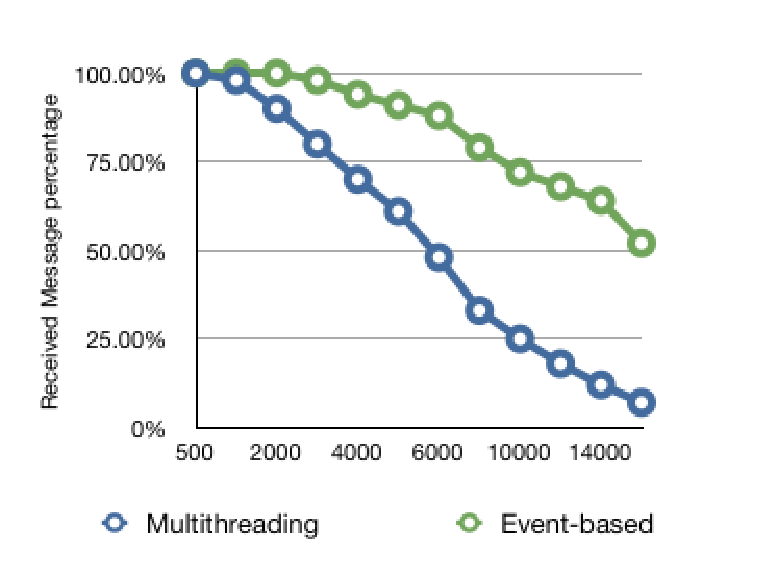
\includegraphics[scale=0.70]{figures/et_rate.eps}
    \caption{Received Message Percentage}
    \label{fig:et_rate}
\end{figure}


\subsection{Extending PushUp Server\\}

\begin{figure}[htb!]
\centering%
    \includegraphics[scale=0.28]{figures/multinode_latency.eps}
    \caption{Mean Publish Trip Time}
    \label{fig:mt_latency}
\end{figure}

\begin{figure}[htb!]
\centering%
    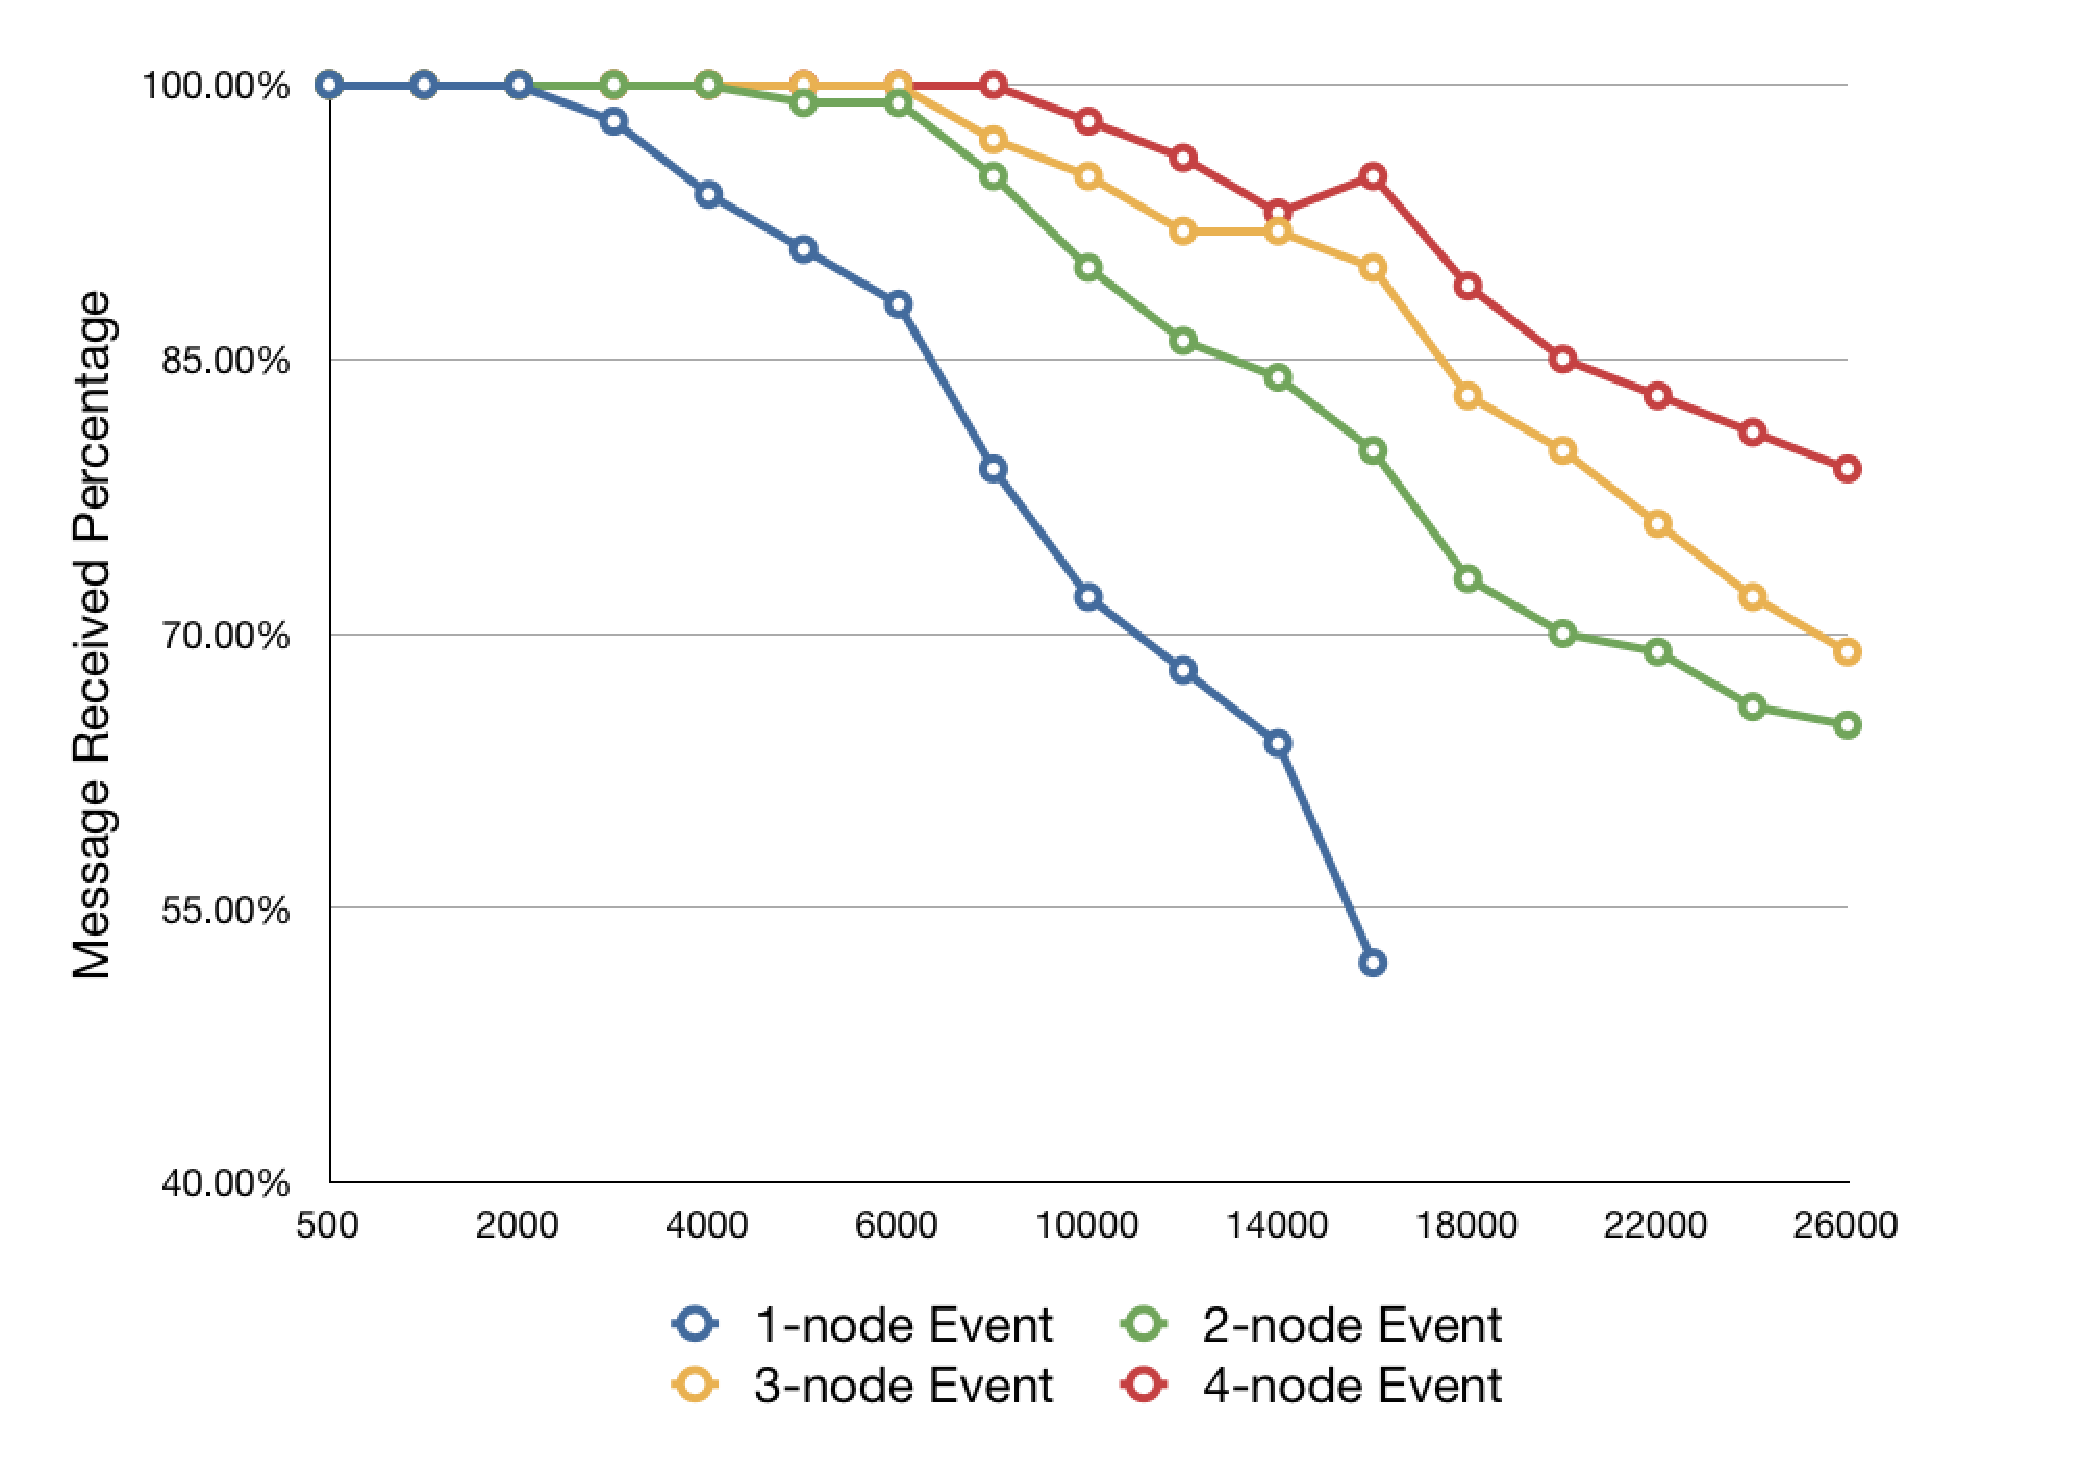
\includegraphics[scale=0.28]{figures/multinode_rate.eps}
    \caption{Received Message Percentage}
    \label{fig:mt_rate}
\end{figure}

As we saw the advantages of PushUp over other event notificaition methods, 
now we would like to extend one PushUp server to $2$,  $3$ and $4$ servers
and see the performance changes as PushUp scales.

In this evaluation, the incoming polling requests will be (almost) evenly 
distributed to each PushUp server. A simple round-robin will be sufficient 
for this task. We used the HAProxy\cite{HAProxy} as a load balancer, which
simply balances the load in the TCP layer.

Figure \ref{fig:mt_latency} and figure \ref{fig:mt_rate}, respectively, show
the {\bf mean publish trip time} and {\bf received message rate} of the 
PushUp servers with different nodes.

These figures verify that the PushUp servers scale almost linearly as the 
number of nodes increases, with a very small overhead in load balancing 
and updates propagation among PushUp servers. 

We can observe in Figure \ref{fig:mt_latency}
that by using 2 nodes instead of 1 node, the MPT for any fixed number of concurrent
connections approximately halves. If 4 PushUp nodes are used instead of 2, then
the MPT is halved again.

